A replacement portal monitor has been designed for layered polymeric films that effectively utilize the \iso[6]{Li} in the detector material. 
An example of the an optimized geometry is shown in \autoref{fig:EXSumDemoLiFZnS} in which the films are \SI{100}{\um} thick placed in a wavelength shifter.
\begin{figure}
  \centering
  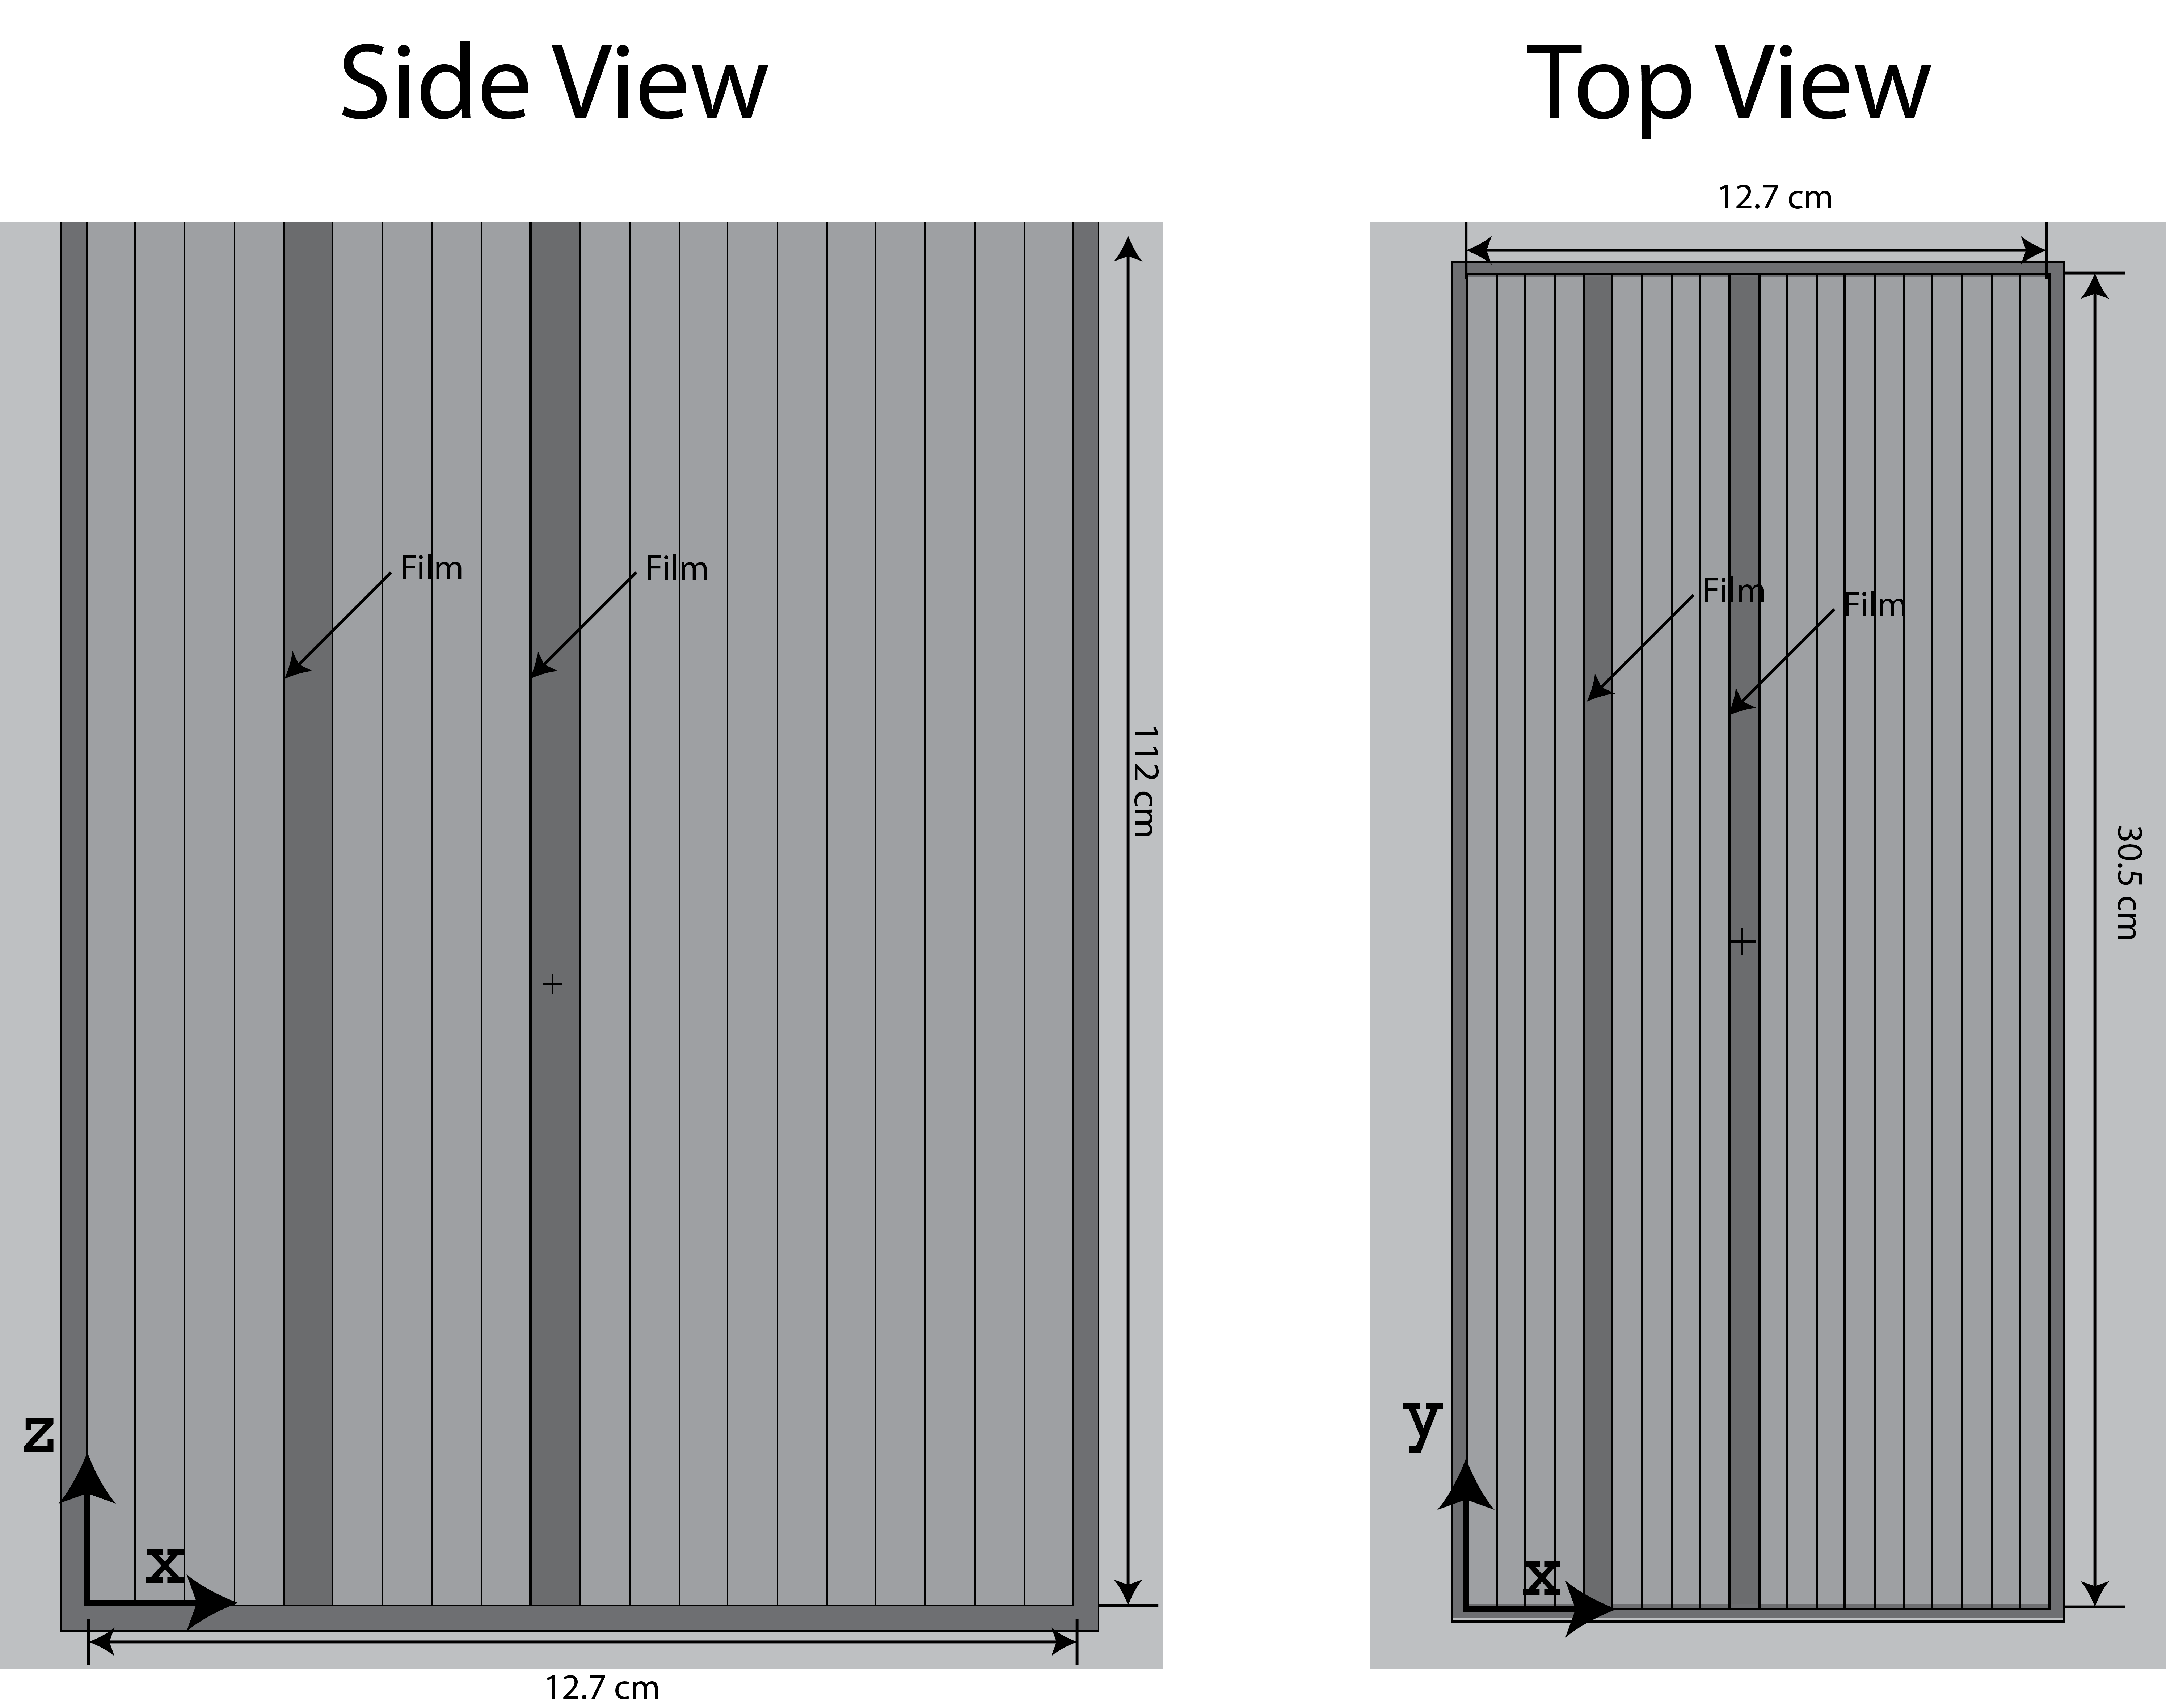
\includegraphics[width=\textwidth]{RPM8OptLayered_LiFZnSBW}
  \caption[]{Example geometry of a film inside the radiation portal monitor. The film material is \iso[6]{LiF} loaded ZnS:Ag, which has a high loading of \iso[6]{Li}. The origin is shown in the lower left of each figure, along with the axis.}
  \label{fig:EXSumDemoLiFZnS}
\end{figure}
The positions of the films necessary to meet the detector criteria are shown in \autoref{tab:EXSumPerf}.
These layered detector designs consist of \SI{100}{\um}, \iso[6]{Li} fluoride loaded polymers that are encased in \SI{5}{\mm} of a wavelength shifting plastic in addition to a \SI{100}{\um} \iso[6]{LiF} loaded ZnS:Ag commercial scintillator also encased in a wavelength shifter.
The wavelength shifter was assumed to have a material composition similar to that of high density polyethylene, which also served as the moderator.
If two \SI{2}{\in} photomultiplier tubes are placed at the top and bottom of a fishtail light guide mounted on the top and bottom of the detector cabinet, 8\% of the optical photons generated in a 10\% loaded polystyrene film can be collected.
It is assumed for the estimated \SI{5}{\in} PMT photons collected that the light collection efficiency of \SI{5}{\in} PMT can be estimated from the ratio of the \SI{2}{\in} to \SI{5}{\in} light collection efficiency as reported in \cite{pnnl_14283}.
\begin{table}
  \caption[]{Simulated detector performance in a design capable of meeting the DHS / DNDO criteria.}
  \label{tab:EXSumPerf}
  \begin{tabular}{m{4.5cm} m{4cm} m{2cm} m{2cm} }
    \toprule
    Detector Composition & Film Positions & \multicolumn{2}{c}{Estimated Photons Collected} \\
                         &                & \SI{2}{\in} PMT & \SI{5}{\in} PMT \\
    \midrule
    10\% \iso[6]{LiF} polystyrene & \SI{2.54}{\cm}, \SI{3.82}{\cm}, \SI{6.36}{\cm} & 160 & 432 \\
    10\% \iso[6]{LiF} polyethylene naphthalene & \SI{1.90}{\cm}, \SI{3.82}{\cm}, \SI{5.08}{\cm} & 240& 410 \\
    \iso[6]{LiF} loaded ZnS:Ag &\SI{3.17}{\cm}, \SI{6.35}{\cm} & 1,900 & 5,130 \\
    \bottomrule
  \end{tabular}
\end{table}

